\documentclass[conference]{IEEEtran}
\IEEEoverridecommandlockouts
\usepackage{cite}
\usepackage{amsmath,amssymb,amsfonts}
\usepackage{algorithmic}
\usepackage{graphicx}
\usepackage{textcomp}
\usepackage{xcolor}
\usepackage{enumitem}
\usepackage{hyperref}

\def\BibTeX{{\rm B\kern-.05em{\sc i\kern-.025em b}\kern-.08em
    T\kern-.1667em\lower.7ex\hbox{E}\kern-.125emX}}
\begin{document}

\title{Service Provider Web Application}

\author{\IEEEauthorblockN{Jainil Modi , 201701208}
\IEEEauthorblockA{\textit{DA-IICT , Gandhinagar } \\
Gujarat, India \\
201701208@daiict.ac.in}
}


\maketitle

\begin{abstract}
Service Provider, a web application through which customers
can request a service like electrical,plumbing, carpeting, painting,
repairing & maintenance, cleaning, and many more. This project is primarily
focused on providing service to customer’s doorstep.
This application is also provided with a feedback-based
rating facility for the customer so that the quality of
service can be improved. Customers are also able to
complain to the shopkeeper about any service. The
Admin has full control over the system and approves the
registered shopkeeper. This web application is
developed using some advanced technologies which are
in great demand in the IT industry today
\end{abstract}



\section{Introduction}
In today’s life, everyone is engaged with busy schedules and
hectic tasks which make them deviate from family life. If any
problem encounters unexpectedly, it distracts them and
makes them choose over the work they have to accomplish
primarily. It is significant to manage both professional and
family life. In such circumstances, every one of us would
have imagined a kind of house that doesn’t have any fault in
electrical devices, leaks in pipes, and a kind of house which
never face any maintenance issues and every one of us has
thought that life would be much better if no problem arises in
getting service at your doorstep. In such a situation, online
service providers play a vital role in today’s life as it has so
many advantages in our life because it makes our daily life
easy. So, giving an idea to design and develop a system that
provides many different services at your doorstep in just one
click. A System that provides different categories of services
like electrical, plumbing, carpeting, painting, repairing &
maintenance, cleaning, and many more. To make it
comfortable for all the users our system is user-friendly. The
System is flexible as a service can be booked from
anywhere you desire.


\section{Functionalities}
\begin{itemize}
\item Login and Sign Up system - Shopkeeper, Customer,
Technician, Admin.
\item Customers can request a service to hire a
technician.
\item The Customer will get OTP and the technician will
have to enter that OTP to verify that he is doing his
job
\item Complaint from customers
\item Feedback from customers
\item The shopkeeper can view, update any service to
process
\item The shopkeeper can add, update and delete any
technician details
\item The shopkeeper can add, update customer details
\item The shopkeeper can view the customer’s request.
\item The shopkeeper can view the feedback and
complaints from customers.
\item Send a notification/mail to the customer for service.
\item The technician can check the service requested by
the customer
\item Login and Sign Up system - Shopkeeper, Customer,
Technician, Admin.
\item Customers can request a service to hire a
technician.
\item The Customer will get OTP and the technician will
have to enter that OTP to verify that he is doing his
job
\item Complaint from customers
\item Feedback from customers
\item The shopkeeper can view, update any service to
process
\item The shopkeeper can add, update and delete any
technician details
\item The shopkeeper can add, update customer details
\item The shopkeeper can view the customer’s request.
\item The shopkeeper can view the feedback and
complaints from customers.
\item Send a notification/mail to the customer for service.
\item The technician can check the service requested by
the customer
\end{itemize}




\section{User Story}
\begin{enumerate}
\item As a customer I want to log in so that I can authenticate
my profile.
\item As a customer I want to request service so that it will
help to regulate my service.
\item As a customer I want OTP so that I can give OTP to a
technician and it will verify that he is doing his service.
\item As a customer I want a complaint box so that I can issue
my complaint.
\item As a customer I want feedback so that I can increase the
quality of service.
\item As a Shopkeeper I want to log in so that I can
authenticate my profile
\item As a shopkeeper I want to handle customer data so that I
can add, view, update customer details anytime.
\item As a shopkeeper I want to handle technician data so that
I can add, view, update, delete technician details anytime.
\item As a shopkeeper I want feedback from customers so that
I can improve my service.
\item As a shopkeeper I want to see complaints so that I can
resolve complaints ASAP.
\item As a shopkeeper I want to see customer pending
requests so that I can solve customer requests ASAP.
\item As a technician I want to log in so that I can
authenticate my profile
\item As a technician I want to see customer requests so that
I can know about customer’s request details.
\item As an admin I want full access to the system so that I
can manage and control applications.
\end{enumerate}


\section{Design}
The project is developed using a specific software
development lifecycle. I have created a modular design
showing all the functionalities of all end users. Then I have
created UML Models consisting of Use case diagram, Class
diagram, Sequence diagram, and Activity diagram. After
that, I designed the UI using Adobe XD.

\subsection{Technology}
Multiple technologies are used in our system.HTML, CSS,
JavaScript is used for front-end styling of applications. These
languages are used to develop Front End UI. REACT.JS is
used for the front-End UI interface / UI component and to
fetch backend data through API in our application. We used
NODE.JS as a backend runtime environment and
Express.js is used as a backend web application framework
for node.js. Database MongoDB is used to store all the data
of our system.

\subsection{Tools}
AdobeXD is used to create UI. VS code tool is used for
backend and front end programming and to store data in
MongoDB database MongoDB atlas tool is used.
\graphicspath{ {./design/} }
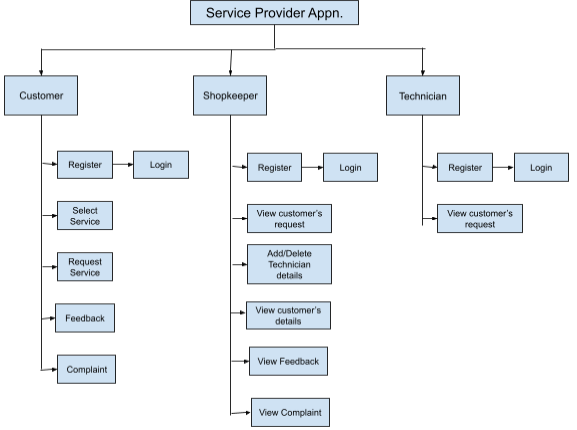
\includegraphics[width=10cm, height=10cm]{design}

\\Web application architecture
\graphicspath{ {./architecture/} }
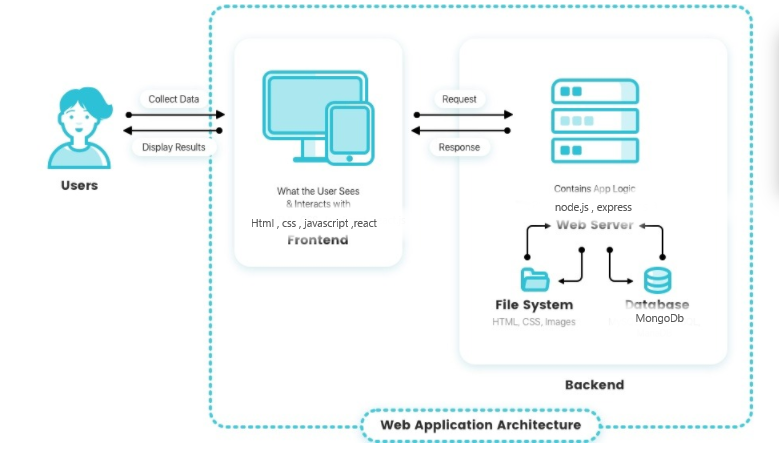
\includegraphics[width=10cm , height=10cm]{architecture}

\\UML Model
\\Use Case Diagram
\graphicspath{ {./usecase/} }
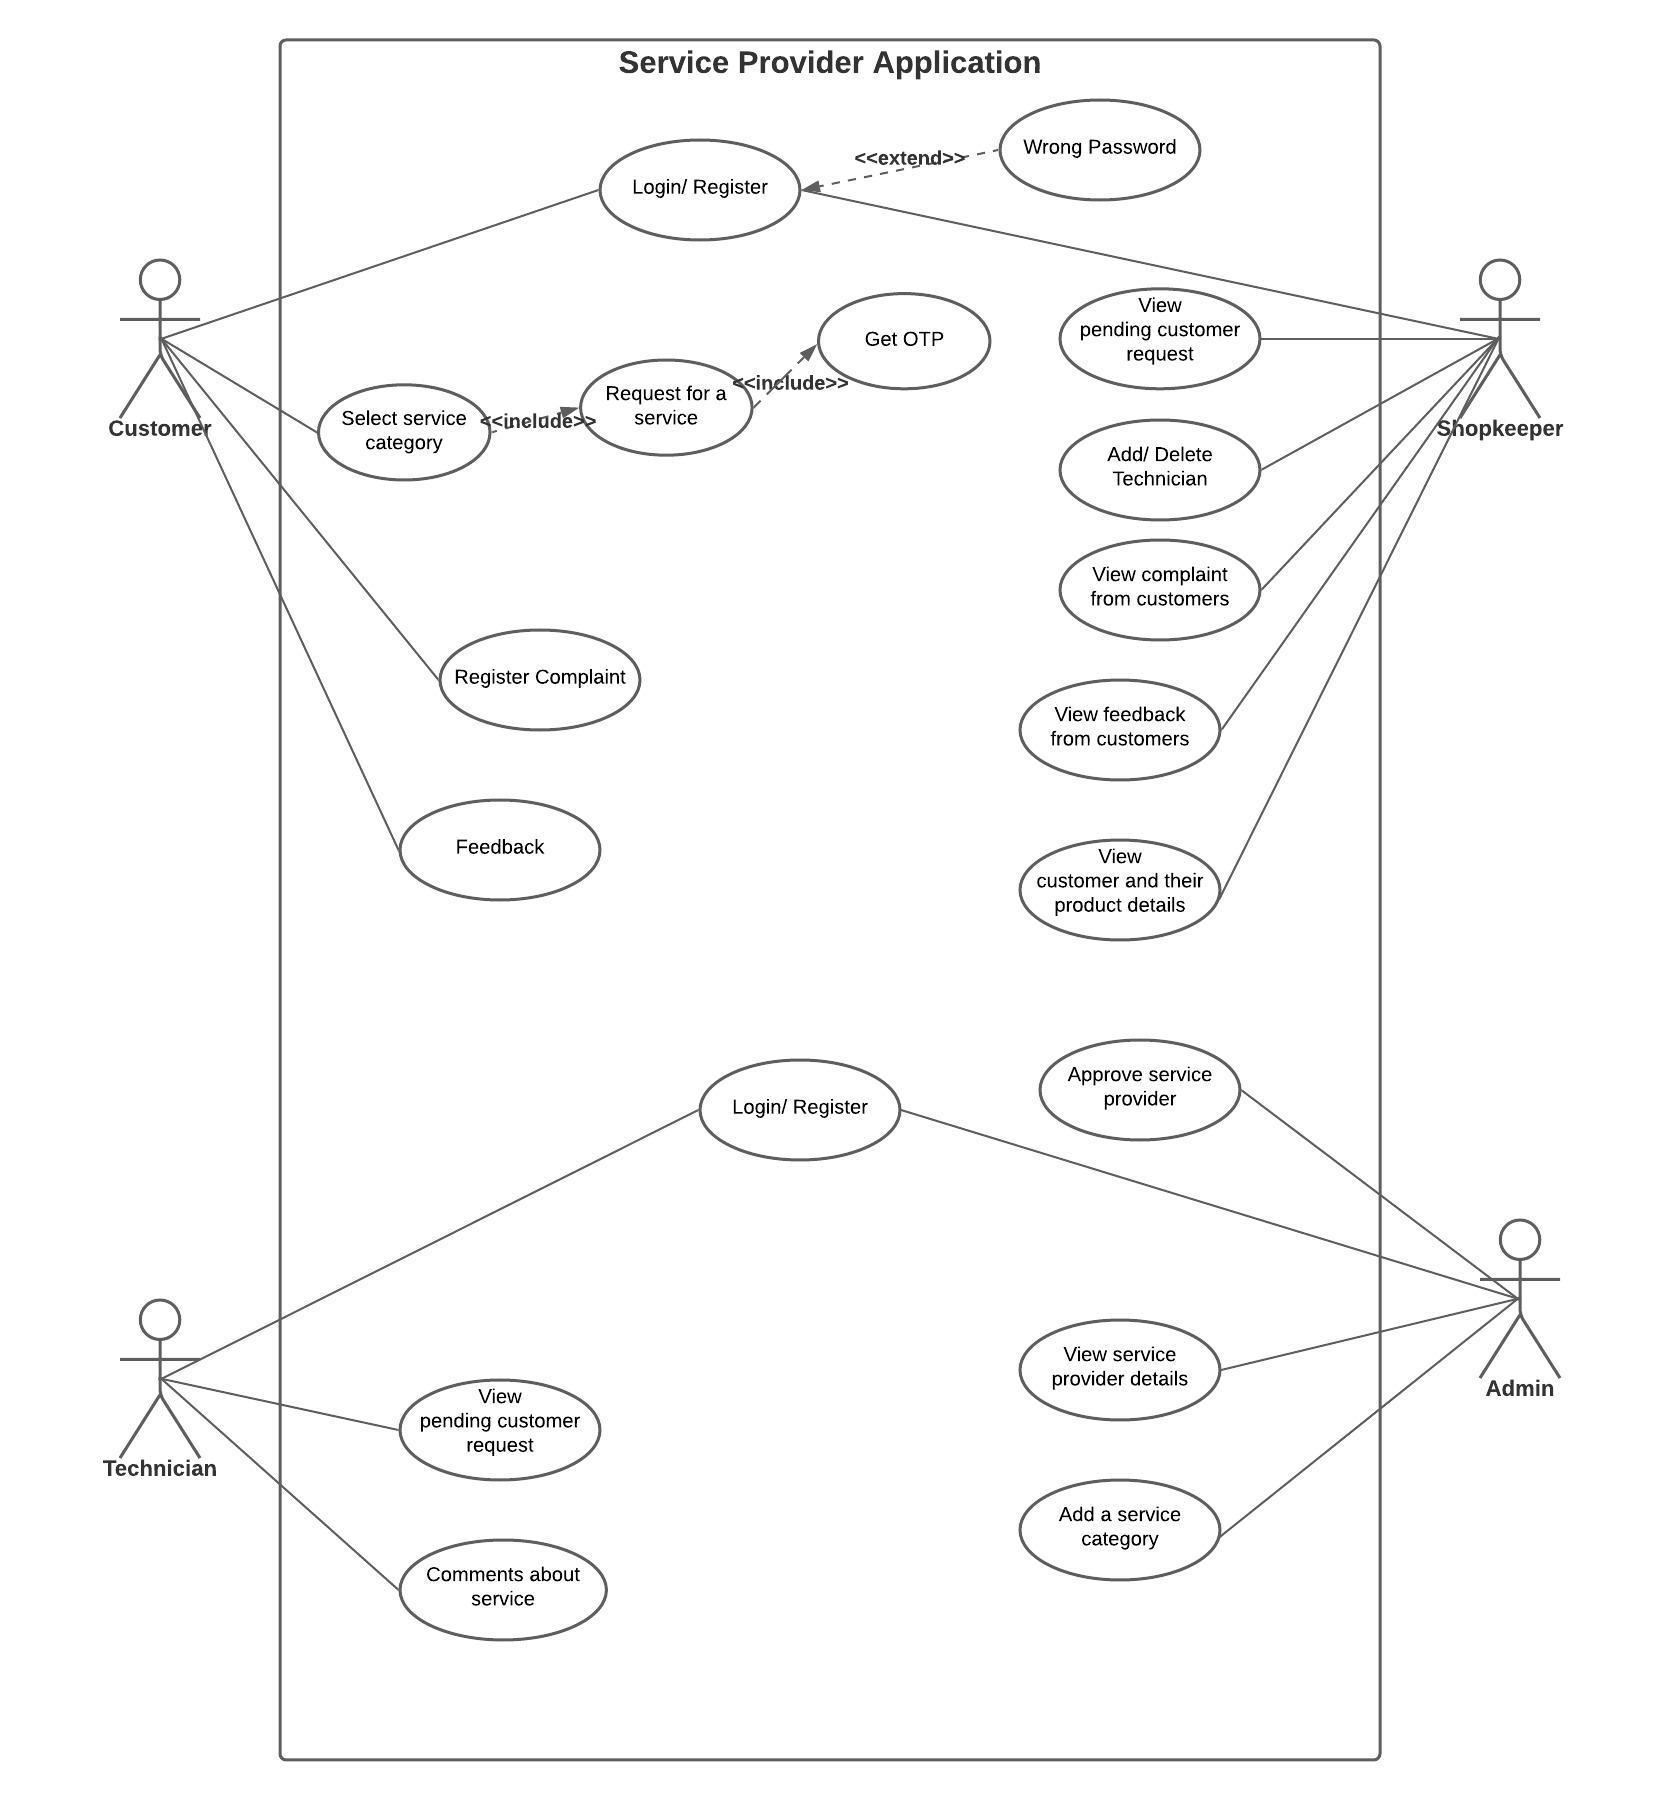
\includegraphics[width=10cm , height=10cm]{usecase}
\\Class Diagram
\graphicspath{ {./class/} }
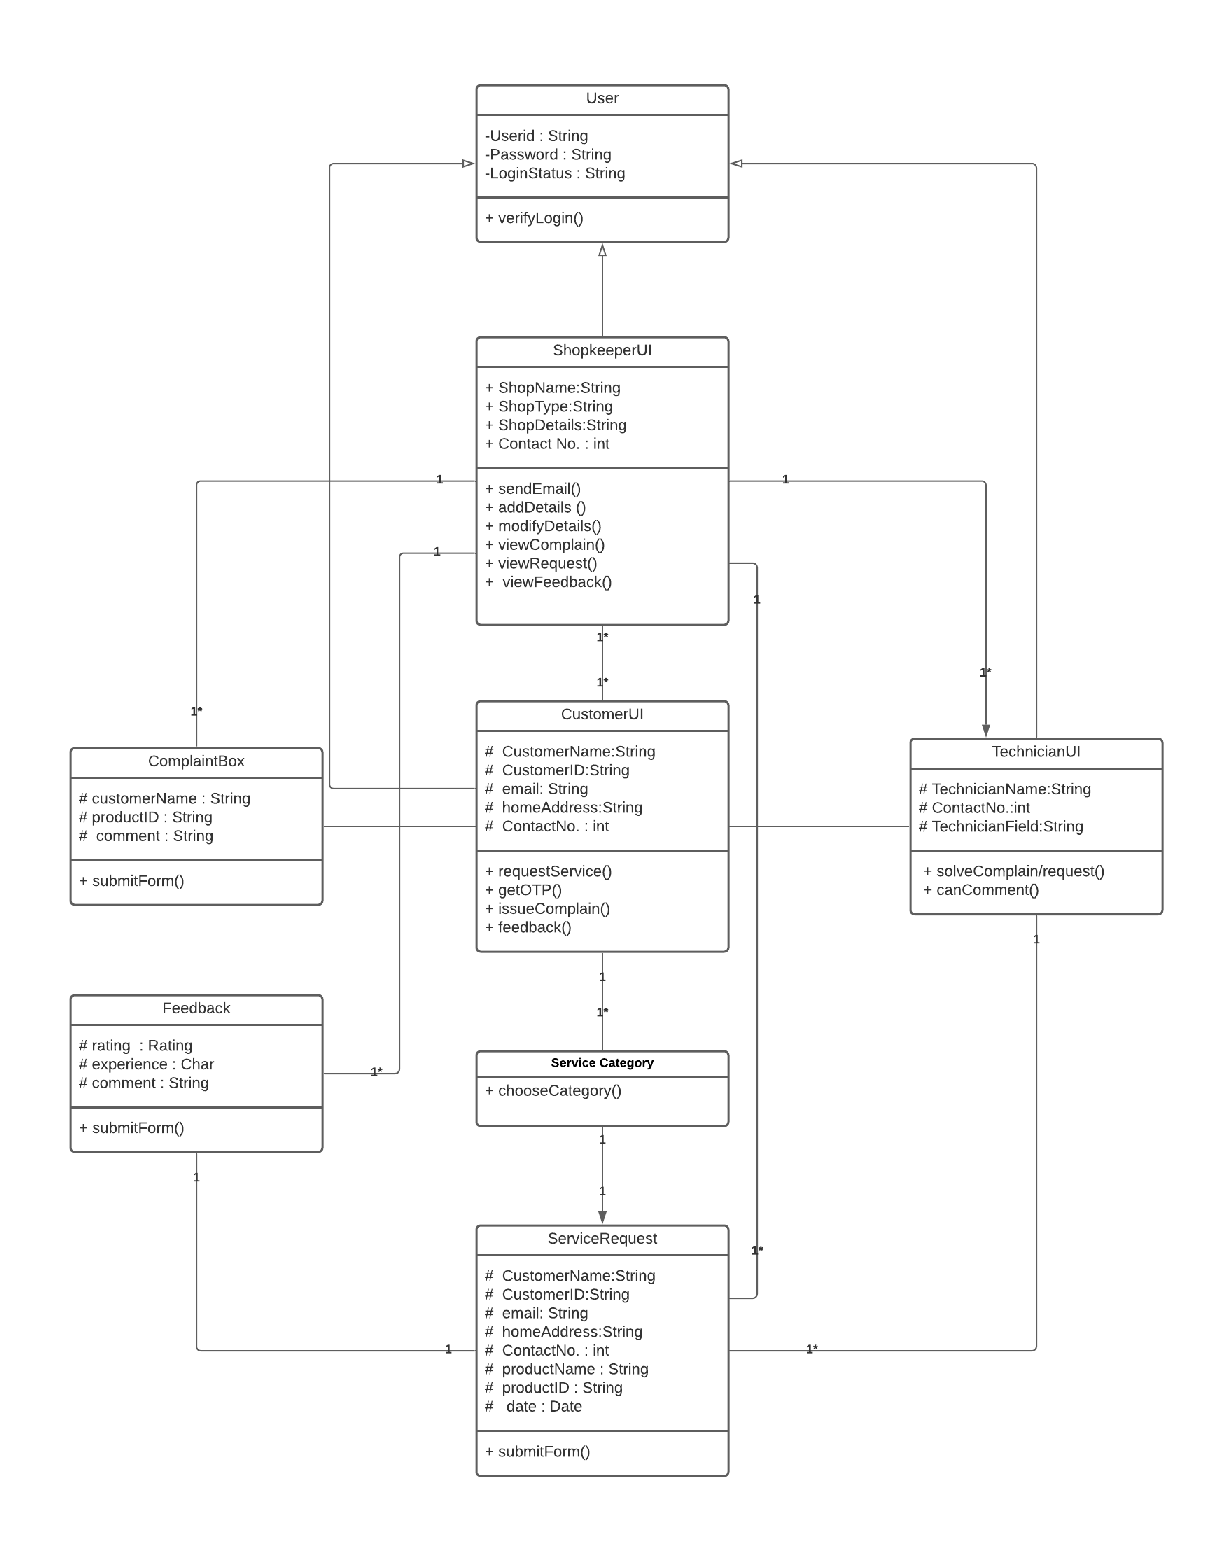
\includegraphics[width=10cm , height=10cm]{class}
\\Sequence Diagram
\graphicspath{ {./sequence/} }
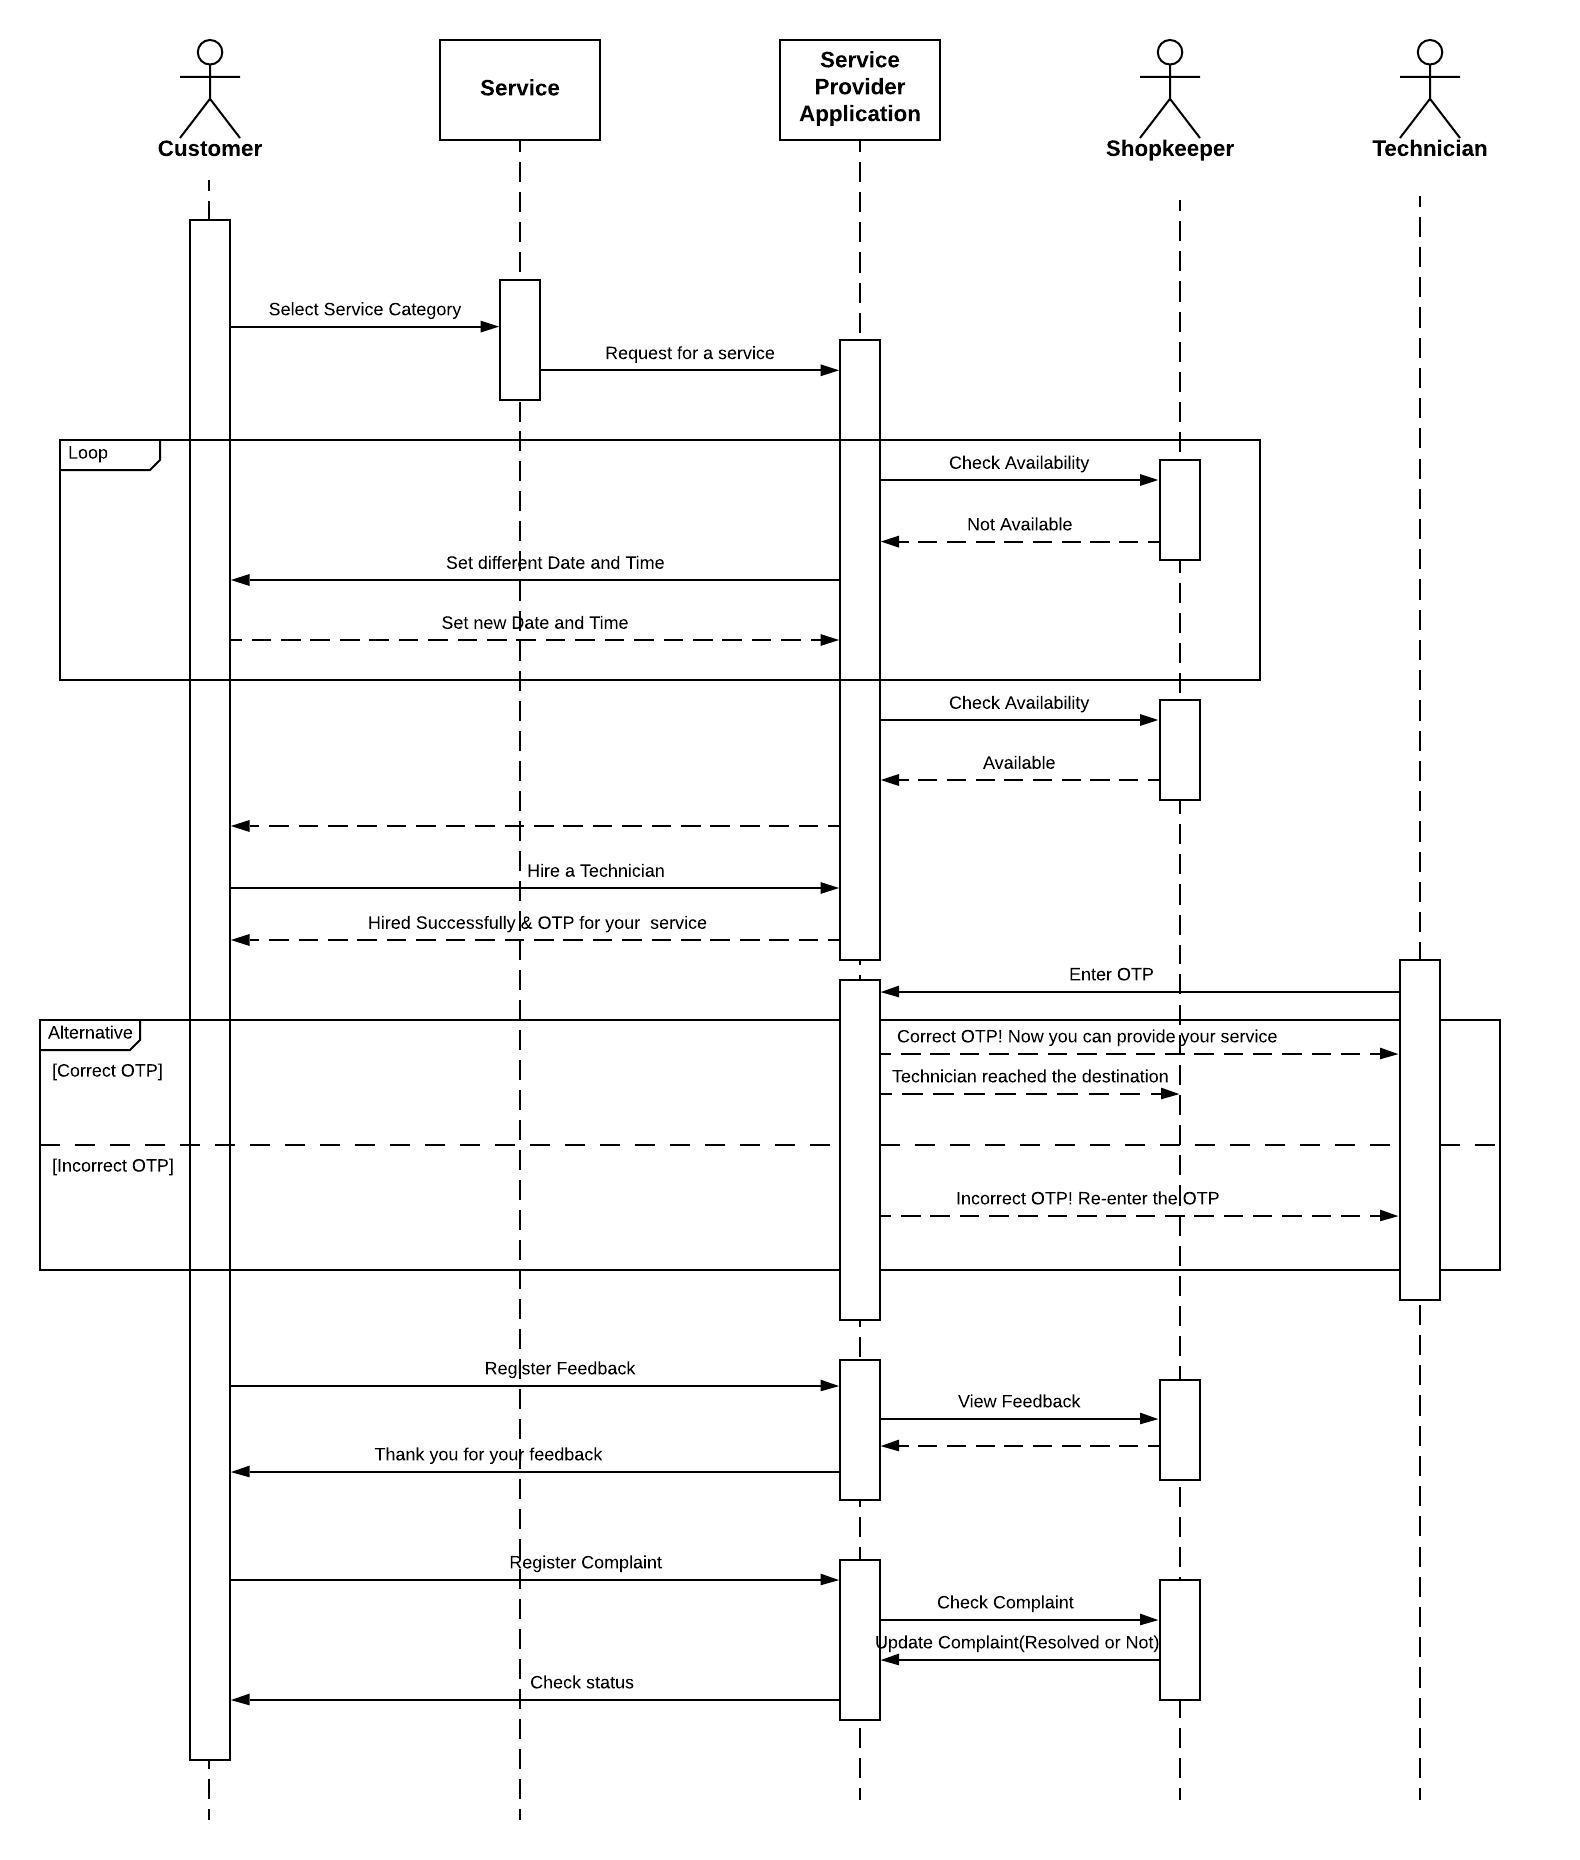
\includegraphics[width=10cm , height=10cm]{sequence}
\\Activity Diagram
\subsection{Shopkeeper}
\graphicspath{ {./shopkeeper/} }
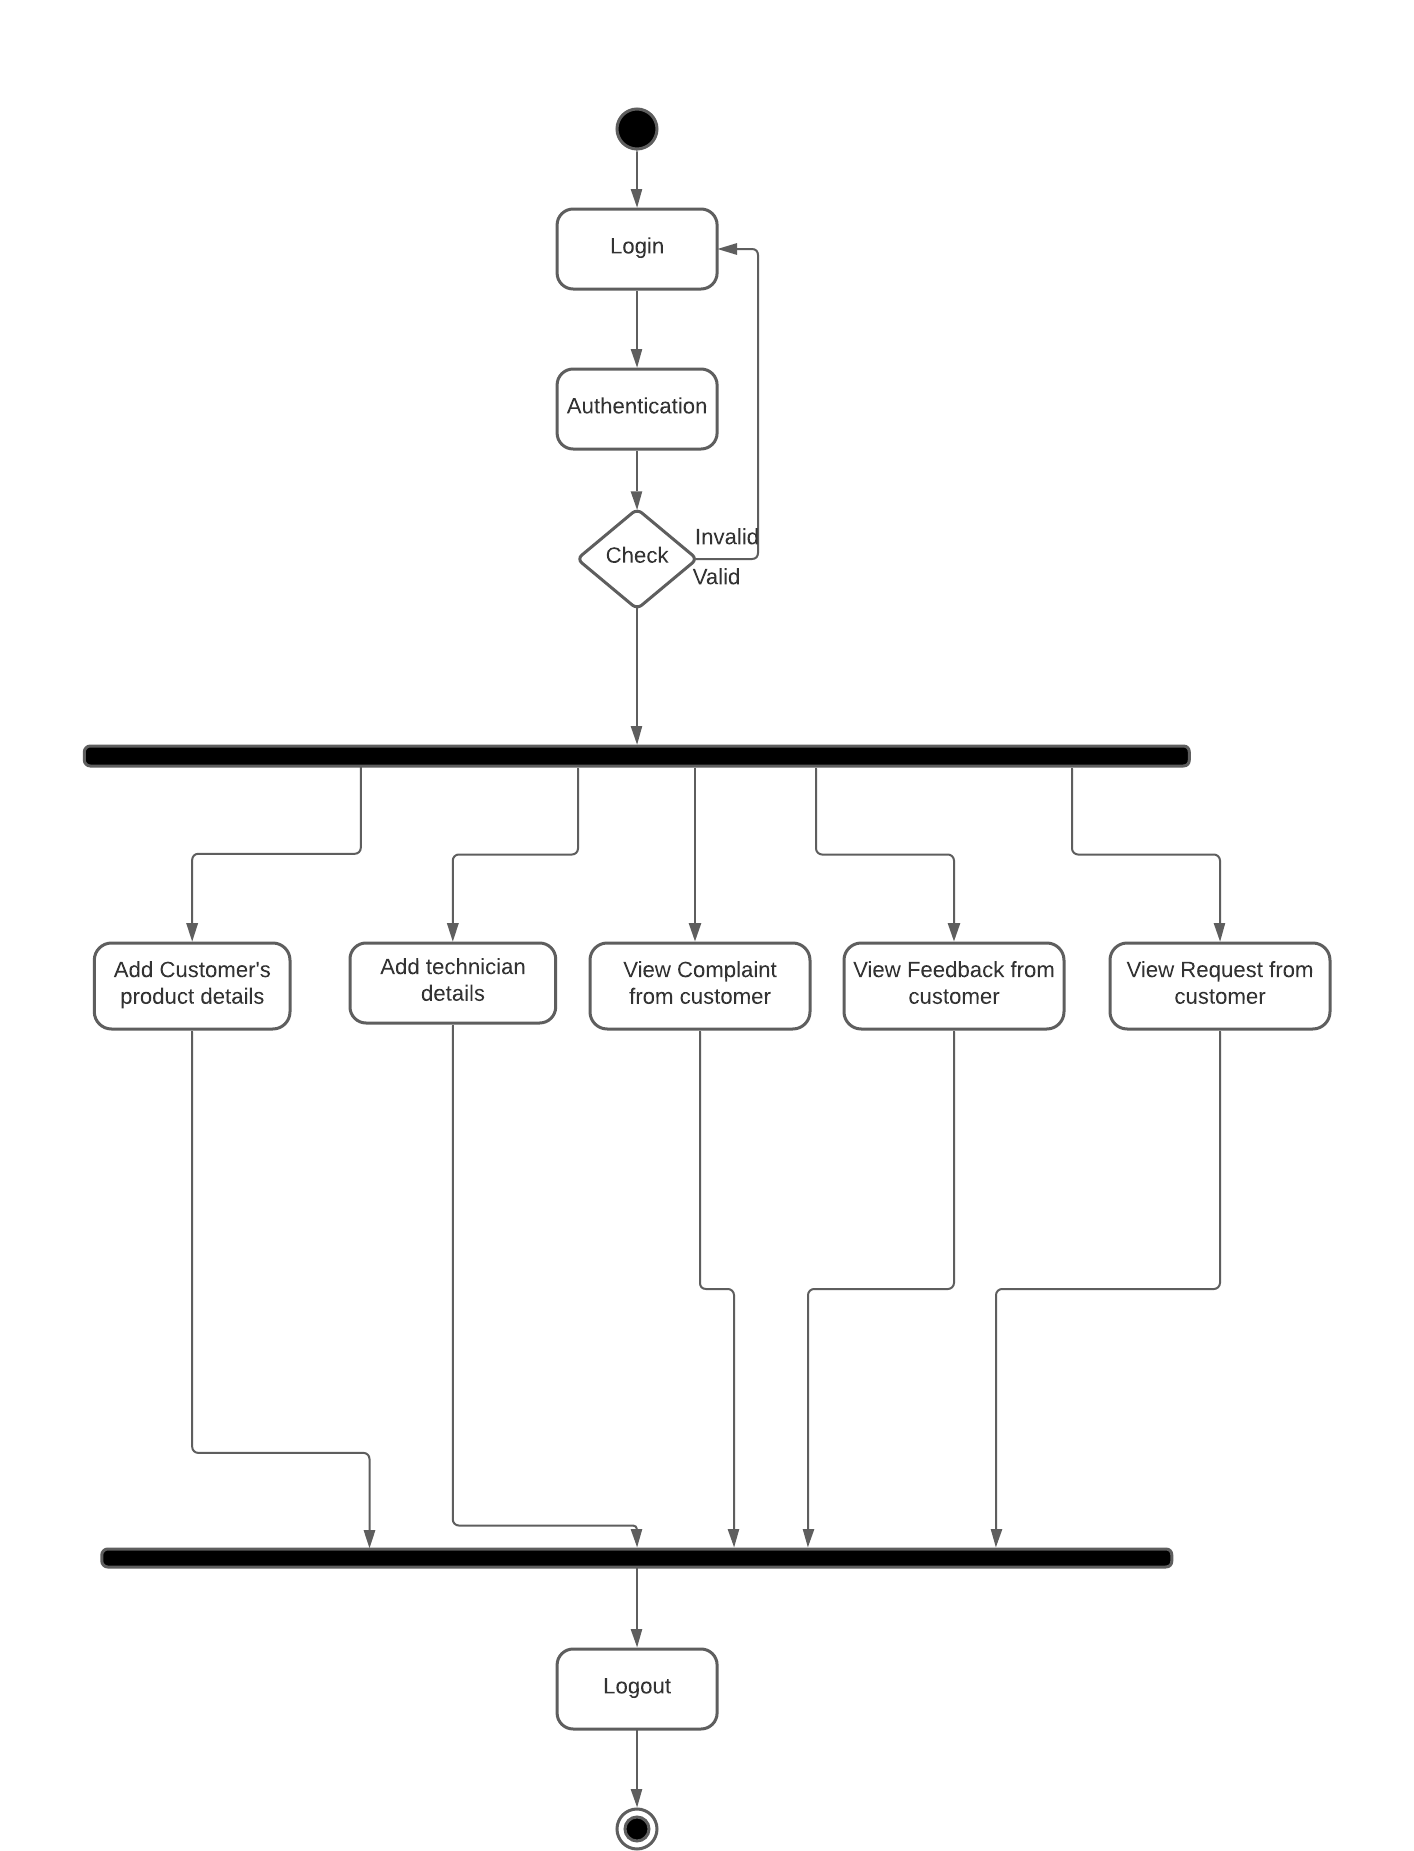
\includegraphics[width=10cm , height=10cm]{shopkeeper}
\\Customer
\graphicspath{ {./customer/} }
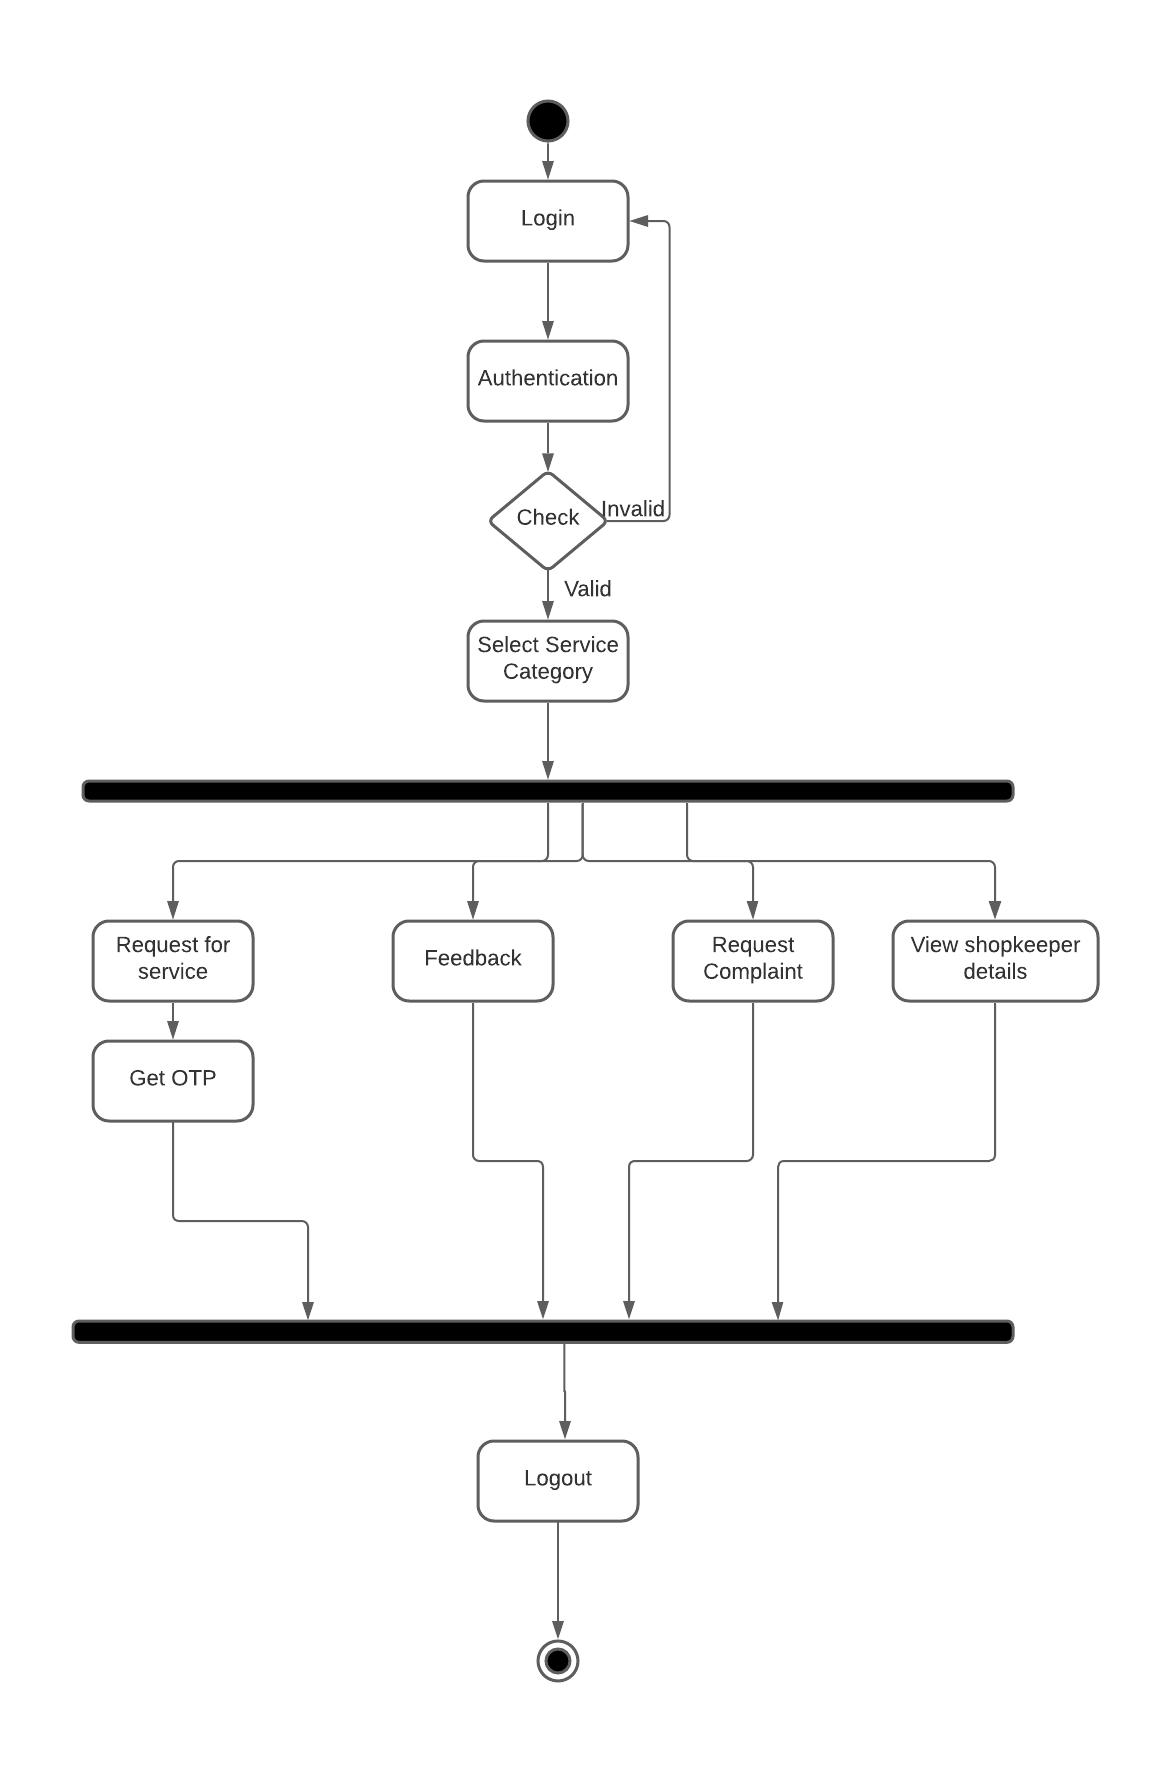
\includegraphics[width=10cm , height=10cm]{customer}



\section{Implementation}
\subsection{sign up/ Log in}
for new users signup page will be open
and if a user is already registered in the application then log
-in page will be opened.
\graphicspath{ {./signup/} }
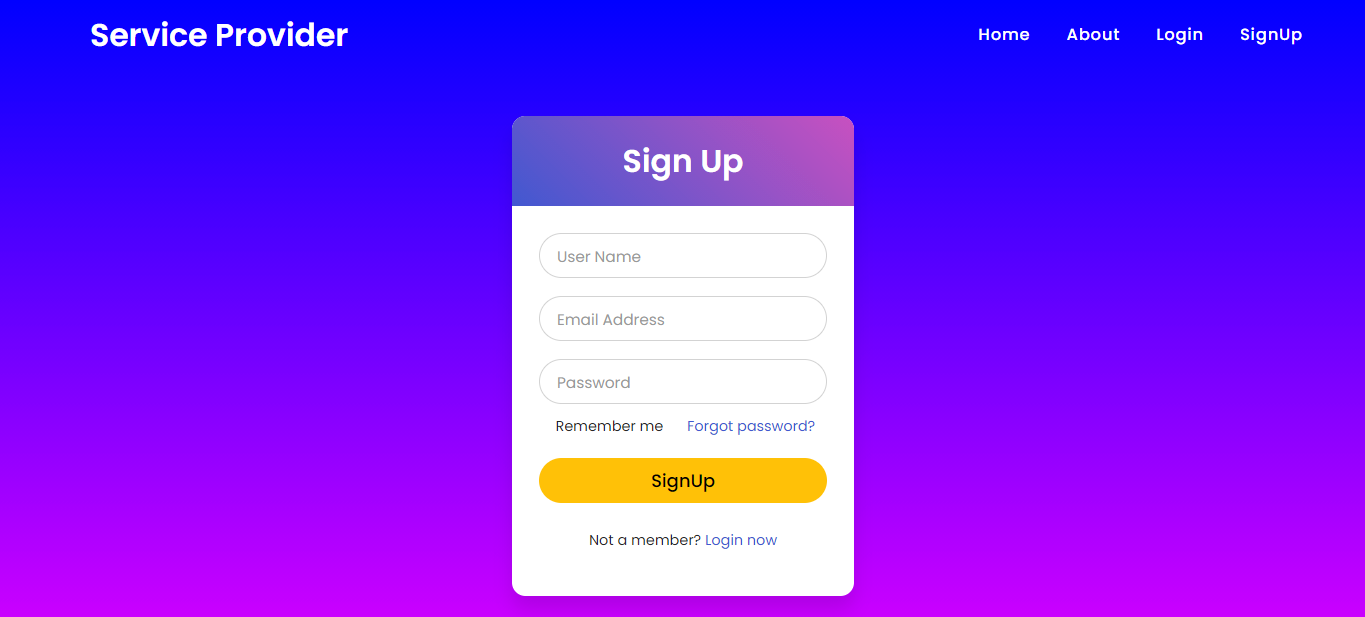
\includegraphics[width=8cm , height=5cm]{signup}

\subsection{userdetails}
when a new user is registered in the
application a unique auto-generated user id will pop up.

\subsection{select service category}
The Customer can select the required service category
\graphicspath{ {./category/} }
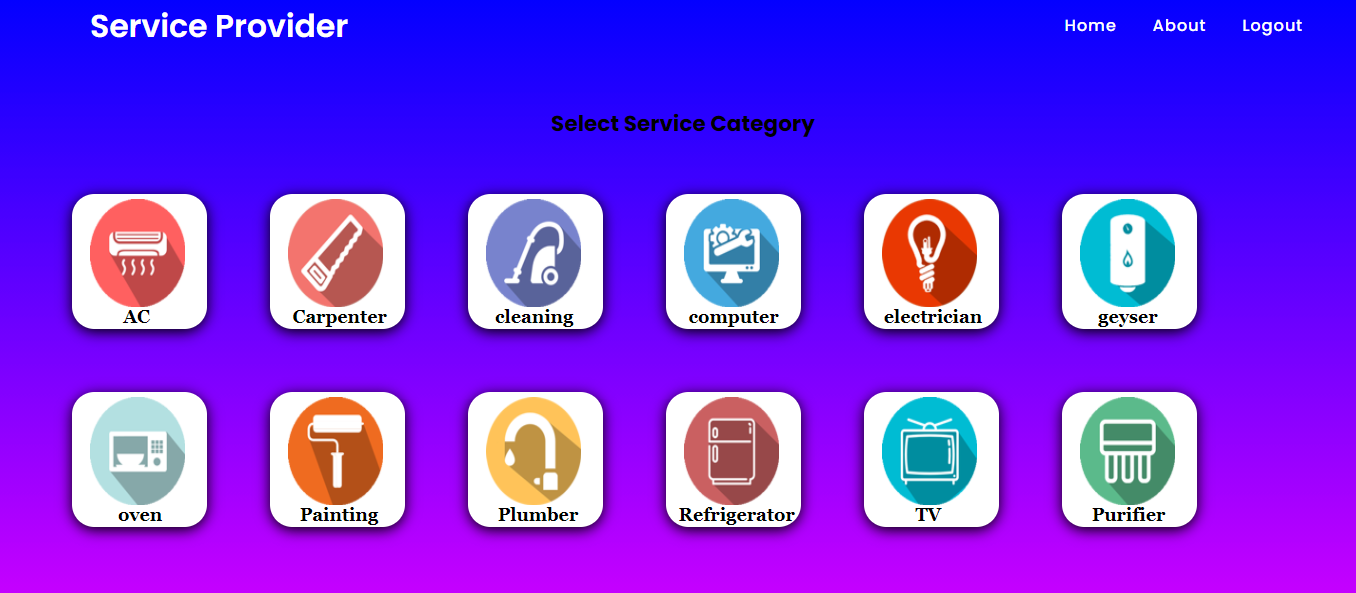
\includegraphics[width=8cm , height=5cm]{category}

\subsection{view shopkeeper details}
Customer can view all registered shopkeeper details like shop name, shopkeeper name, and
shopkeeper id.

\subsection{customer request form}
When customers select a category service request form will be opened. While
submitting the form, a customer request will be sent to the
appropriate shopkeeper.
\graphicspath{ {./request/} }
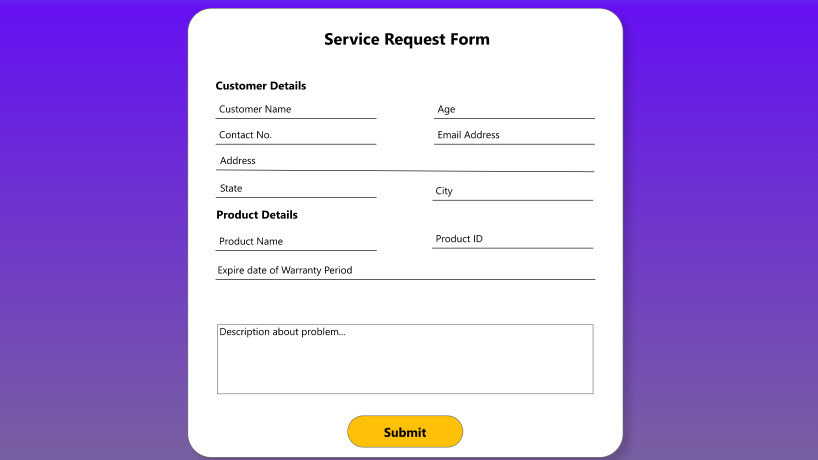
\includegraphics[width=8cm , height=5cm]{request}

\subsection{feedback form}
Customers can give feedback on the service provided by the shopkeeper.
\graphicspath{ {./feedback/} }
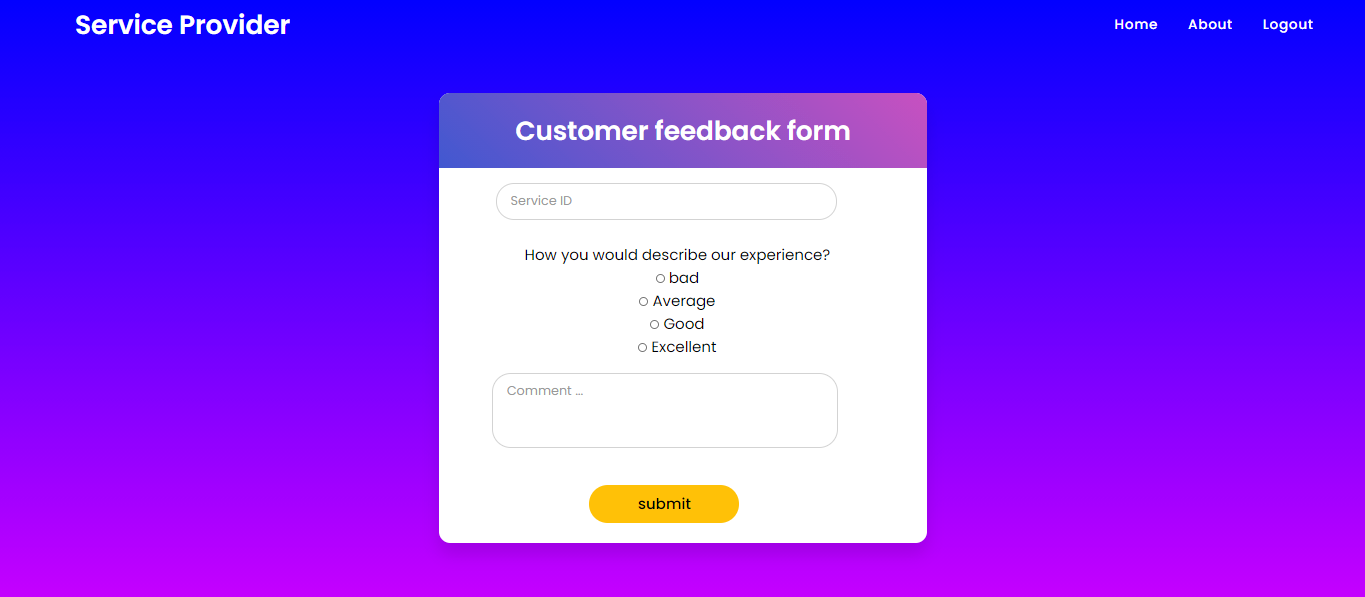
\includegraphics[width=8cm , height=5cm]{feedback}

\subsection{complaint box}
Customers can do complain if he/she is not satisfied with service.
\graphicspath{ {./complaint/} }
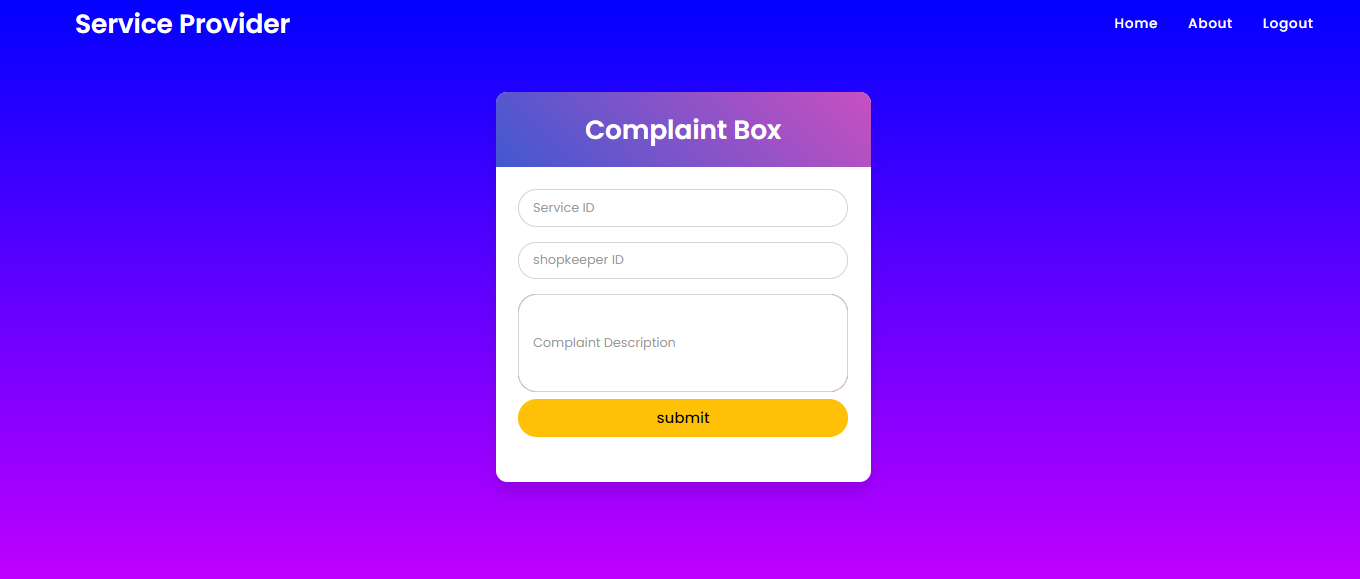
\includegraphics[width=8cm , height=5cm]{complaint}

\subsection{customer details}
Shopkeepers can see customer service requests, feedback, and complaint details.
\graphicspath{ {./details/} }
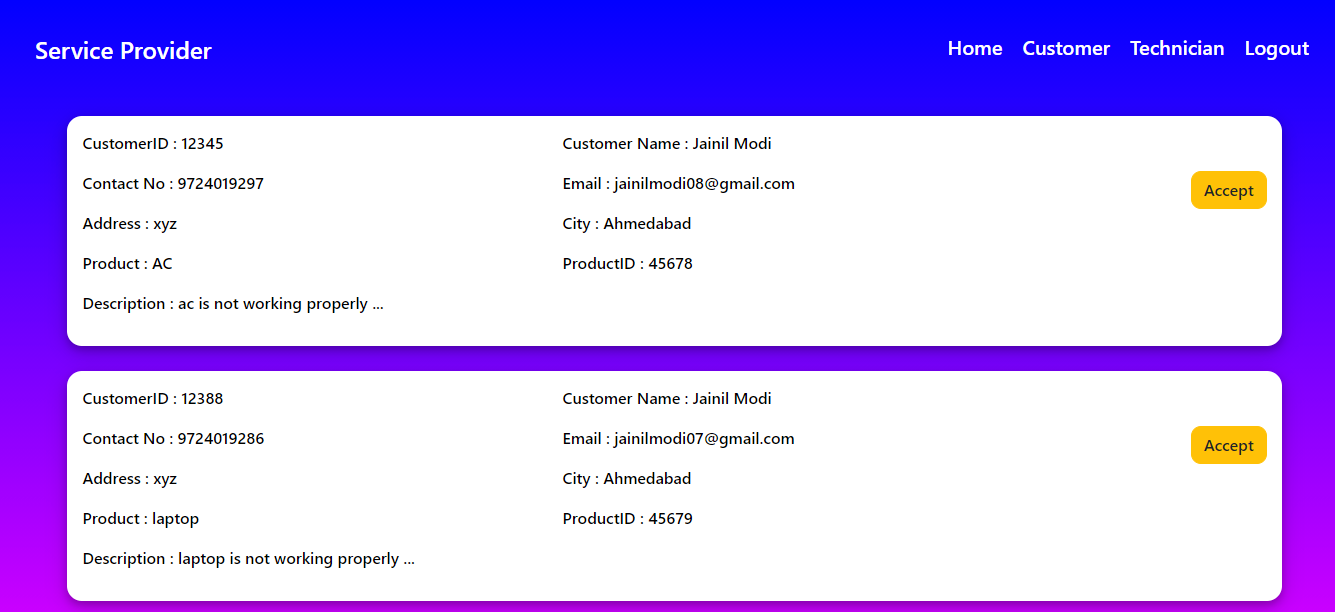
\includegraphics[width=8cm , height=5cm]{details}

\subsection{Add and view Technician and customer Details}
Shopkeepers can add and view technician and customer details.
\graphicspath{ {./viewtech/} }
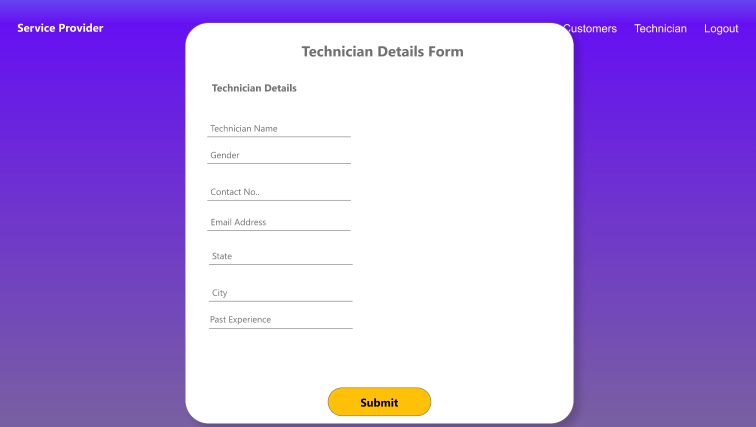
\includegraphics[width=8cm , height=5cm]{viewtech}

\section{Testing}
\begin{enumerate}
\item Login/signup
Test Case ID : TU01
Test Scenario : Check Customer login with valid data
Test Steps : Go to localhost:3000/login
enter email and password
click submit
Test Data : email : guest1@gmail.com
Password : 1234
Expected Results: User should Login successfully
Actual Results : User Login Successfully
Pass/Fail : Pass
Test Case ID : TU02
Test Scenario : Check Customer login with invalid data
Test Steps : Go to localhost:3000/login
enter email and password
click submit
Test Data : email : guest1@gmail.com
Password : 1277
Expected Results : User should not Login successfully
Actual Results : Invalid Credentials
Pass/Fail : Pass
Test Case ID : TU03
Test Scenario : Check Customer login with invalid data
Test Steps : Go to localhost:3000/login
enter email and password
click submit
Test Data : email : guest177@gmail.com
Password : 1234
Expected Results : User should not Login successfully
Actual Results : Invalid Credentials
Pass/Fail : Pass

\item serivce request form
If registered shopkeeper id is : 65778
Test Case ID : TU04
Test Scenario : Check if Customer enter with valid data
then respective shopkeeper can see his/her customer
request
Test Steps : Go to localhost:3000/customerform
enter all details
click submit
Go to localhost:3000/request
Test Data : Customer ID : 16678
Customer Name : guest2
Product ID : 123M
Product Name : AC
Shopkeeper ID : 65778
Expected Results : User should submit successfully and
shopkeeper can see his/her request details .
Actual Results : Form submitted Successfully
Pass/Fail : Pass
Test Case ID : TU05
Test Scenario : Check if Customer enter with Invalid data
Test Steps : Go to localhost:3000/customerform
enter all details
click submit
Go to localhost:3000/request
Test Data : Customer ID : 16678
Customer Name : guest2
Product ID : 123M
Product Name : AC
Shopkeeper ID : 65789
Expected Results : User should not submit successfully
Actual Results : enter valid details
Pass/Fail : Pass


\item customer feedback form
Test Case ID : TU06
Test Scenario : Check if Customer enter with valid data
Then the respective shopkeeper can see his/her feedback
details.
Test Steps : Go to localhost:3000/feedbackform
enter all details
click submit
Go to localhost:3000/feedbacks
Test Case ID : TU06
Test Scenario : Check if Customer enter with valid data
Then the respective shopkeeper can see his/her feedback
details.
Test Steps : Go to localhost:3000/feedbackform
enter all details
click submit
Go to localhost:3000/feedbacks

\item customer complaint box
Test Case ID : TU08
Test Scenario : Check if Customer enter with valid data
Then the respective shopkeeper can see his/her complaint
details
Test Steps : Go to localhost:3000/complaintform
enter all details
click submit
Go to localhost:3000/complaints
Test Data : Shopkeeper ID : 65778
Service ID : 78998
Comment : service was not good.
Expected Results : User should submit successfully and
shopkeeper can see his/her complaint details
Pass/Fail : Pass
Test Case ID : TU09
Test Scenario : Check if Customer enter with invalid data
Test Steps : Go to localhost:3000/complaintform
enter all details
click submit
Go to localhost:3000/complaints
Test Data : Shopkeeper ID : 65999
Service ID : 78998Comment : service was not good.
Expected Results : enter valid details
Pass/Fail : Pass

\end{enumerate}

\section{Results and Discussions}
A functional web application in which customers have to log
in first. Then they can request a particular service. This
request goes to the shopkeeper and technician dashboard.
Shopkeepers can manage the details of technicians.
Customers can also give feedback and complaints about any
service. Shopkeepers can view feedback and complaints
from the customer so that they can improve their services.
To verify, the technician is doing his job or not, there is an
OTP system in which the customer will receive the OTP and
it will be shared with the technician only when he goes to do
his job

\section{Conclusion}
A service provider web application is developed which helps
in online service booking. Service Provider application is the
new trend in the market of on-demand applications. Although
services like UrbanClap, Handyman, and Taskrabbit are
already existing in the market; there are still many
possibilities that we can explore and execute. With proper
market research, the inclusion of vital features, user’s needs,
followed by appropriate marketing can make your app
successful.

\section{future work}
In the future, we can develop a web application in which we
will put map navigation for the technician to find the location
of the customer and also for the customer to track the
technician using GPS. We can also add payment methods to
our system so that the customers can pay online.

\section{References}
\begin{itemize}
\item \href https://developer.mozilla.org/en-US/
\item \href https://getbootstrap.com/
\item \href https://www.w3schools.com/
\item \href https://ejs.co/
\item \href https://nodejs.org/en/
\item \href https://expressjs.com/

\end{itemize}

\end{document}
